

\subsection{1.19 Строение соединений переходных металлов в высших и низших степенях окисления. Изомерия комплексных соединений.}
Все переходные металлы являются типичными металлами, атомы способны легко окисляться и быть в положительном валентном состоянии, есть много соединений, где валентное состояние считается нулевым.
Общая характеристика:
\begin{itemize}
	\item Существуют координационные соединения и комплексы
	\item $E_{\text{связи}}$ при движении вниз растёт
	\item Высокая ЭО среди металлов
	\item $d$-оболочка хорошо поляризуема 
	\item Самые распространенные степени окисления: $+2$, $+3$
	\item Большая устойчивость соединений тяжелых $d$-металлов в высших степенях окисления
	\item $4d$ и $5d$ элементы имеют большие координационные числа, чем $3d$ элементы
\end{itemize}
\begin{figure} [H]
	\centering {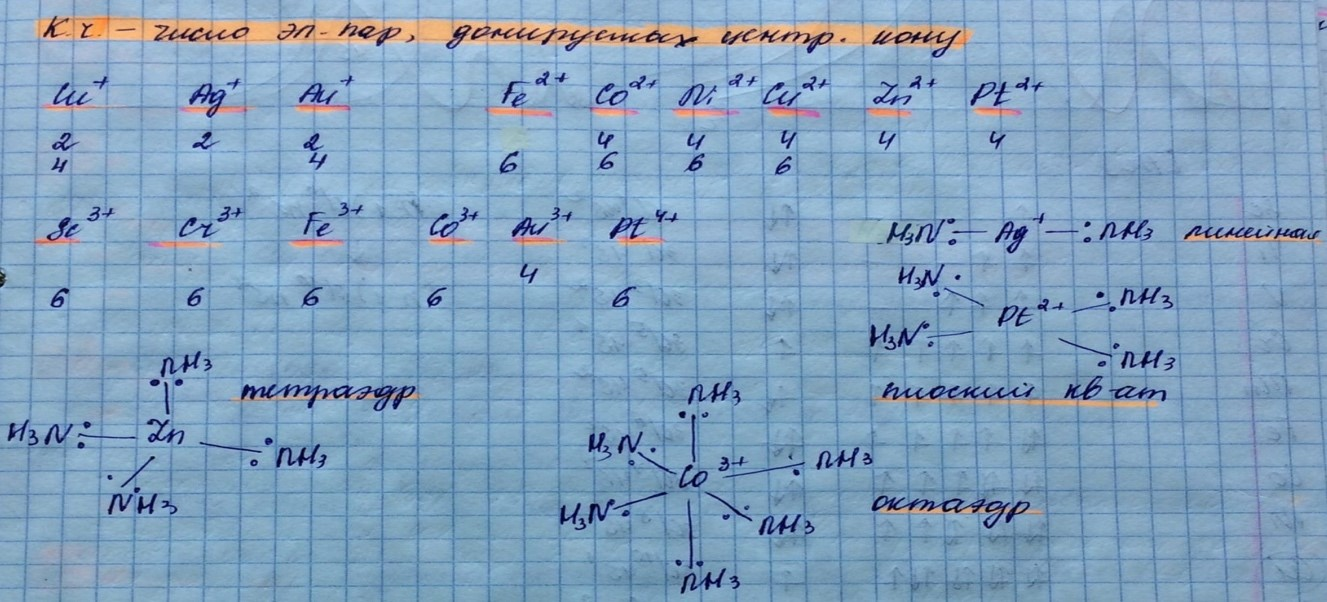
\includegraphics[scale=1.2]{qq1}}
\end{figure}
Электронные конфигурации:
\begin{figure} [H]
	\centering {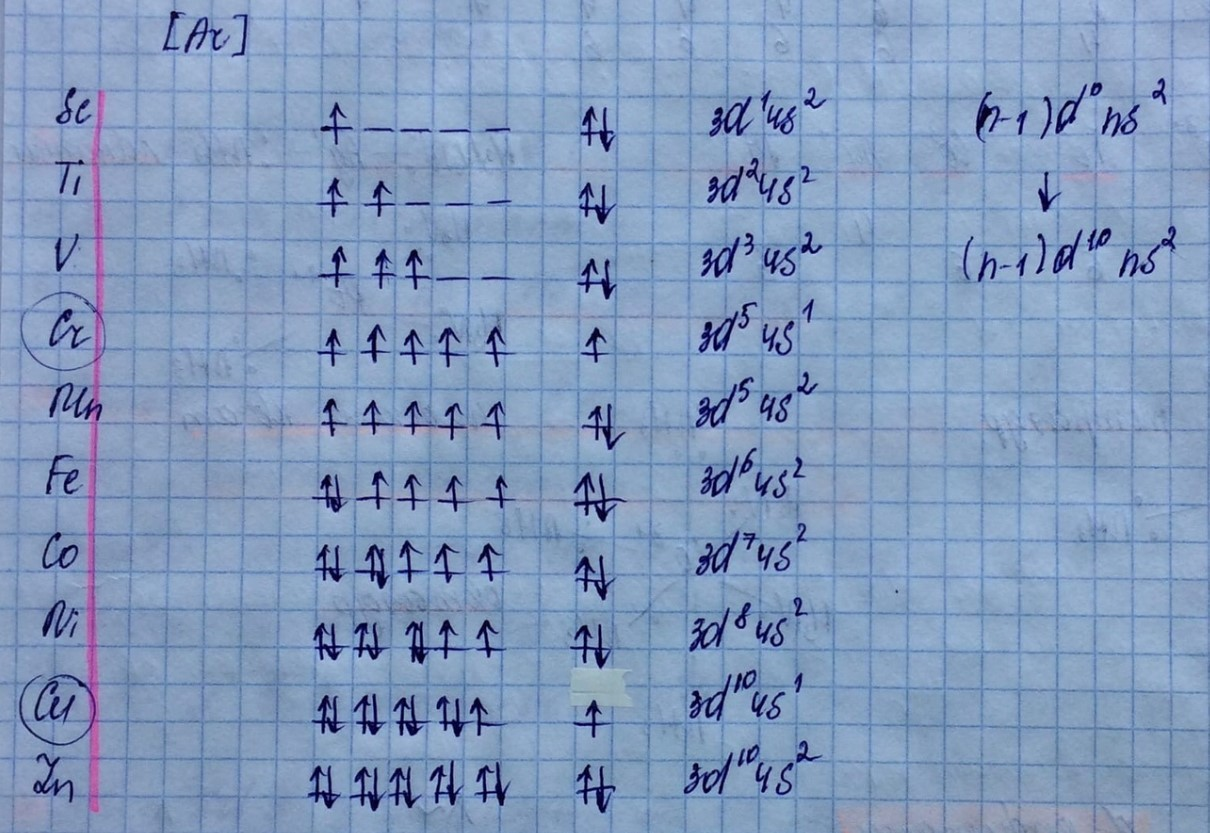
\includegraphics[scale=0.8]{qq2}}
\end{figure}
Возможно образование четкого октаэдрического поля.  
\[
M^{2+} + 6H_2O = \left[M(H_2O)_6\right]^{2+}
\]
Отсюда и происходит термин «кристаллическое поле». 
\begin{figure} [H]
	\centering {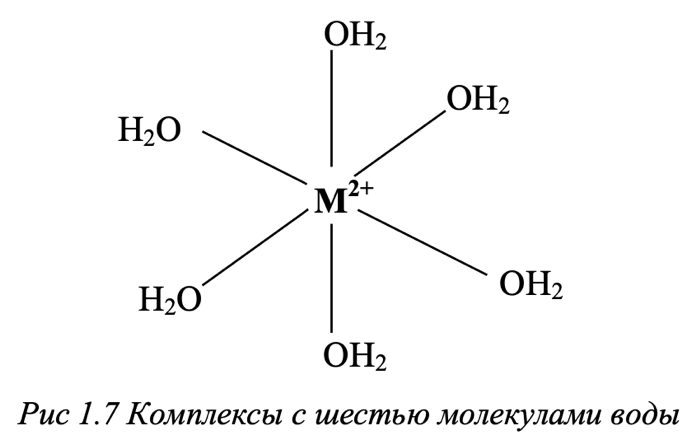
\includegraphics[scale=0.9]{qq3}}
\end{figure}
Если вокруг металла четыре лиганда, кристаллические поля могут быть в форме квадрата или тетраэдра. Если шесть, то кристаллическое поле октаэдрическое, такие соединения больше всего распространены. 
\begin{figure} [H]
	\centering {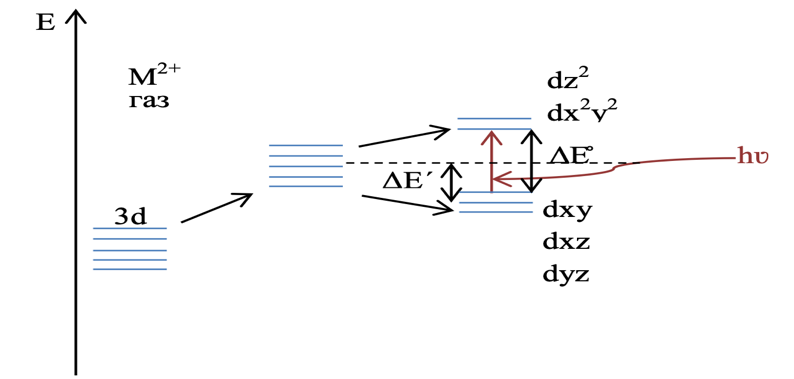
\includegraphics[scale=1.5]{qq4}}
\end{figure}
Происходит расщепление $d$ орбитали на две группы: три орбитали уходят вниз, а две – вверх. Центр тяжести остается на месте. Вниз уходят $d_{xy}$, $d_{xz}$, $d_{yz}$, те, которые между лигандами. \\
Вверх уходят $d_{z^2}$, $d_{x^2 -y^2}$. Если электронов не много, они все должны оказаться внизу. $\Delta E$ - общее расщепление, связано с тем, насколько сильно лиганды поляризуют. Некоторые лиганды расщепляют слабее, некоторые - сильнее (согласно стереохимическому ряду).
\begin{flushleft}
	\begin{figure} [H]
	\centering {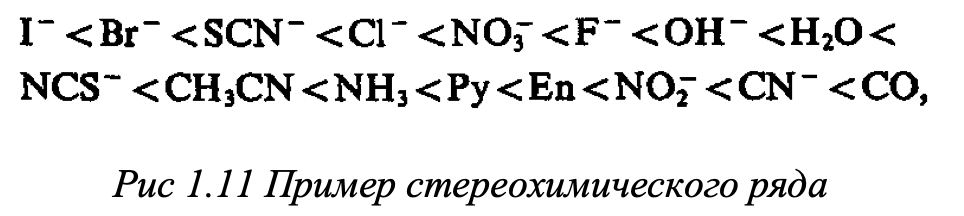
\includegraphics[scale=1]{qq5}}
\end{figure}
\end{flushleft}
\textbf{Изомерия комплексных соединений:} \\
\begin{itemize}
	\item Ионизационная изомерия: \\
	Темно-красное $\left[Co(NH_3)_5 Br \right]SO_4$ и красное $\left[Co(NH_3)_5SO_4 \right]Br$ при диссоциации в воде дают различные анионы: первое - $SO^{2-}_4$, второе - $Br^-$
	\item Cольватная (гидратная) изомерия: \\ 
	Осуществляется при участии нейтральных молекул растворителя и заключается в перераспределении их молекул между внутренней и внешней сферой комплексного соединения. Например три изомера гидратированного хлорида хрома:
	\begin{itemize}
		\item серо-голубой $\left[ Cr(H_2O)_6Cl_3  \right] $ 
		\item светло-зеленый $\left[ Cr(H_2O)_5Cl  \right]Cl_2 \cdot H_2O$ 
		\item темно-зеленый цис-$\left[ Cr(H_2O)_4Cl_2  \right]Cl \cdot 2H_2O$ 
	\end{itemize}
	\item Координационная изомерия: \\
	 Характерна для соединений с комплексными катионами и анионами и проявляется во взаимном обмене лигандами между катионами и анионами. \\
	 Примерами являются:
	 \begin{itemize}
	 	\item $\left[ Co(NH_3)_6  \right] \left[ Cr^{III}(CN_6)\right]$ и $\left[ Cr(NH_3)_6  \right] \left[ Co^{III}(CN_6)\right]$
	 	\item $\left[ Cu(NH_3)_4  \right] \left[ PtCl_4\right]$ (фиолетовый) и $\left[ Pt(NH_3)_4  \right] \left[ CuCl_4\right]$ (зеленый)
	 \end{itemize}
	\item Проявление амбидентатности: \\
	Этот тип изомерии обусловлен наличием лигандов, способных образовывать связи через разные донорные атомы (такие лиганды называют амбидентатными). Например красный и желтый изомеры комплекса $ \left[ Co(NH_3)_5(NO_2) \right]Cl_2 $ причем в первом из них лиганд $NO_2^-$ координирован через атом кислорода ($Co-ONO^-$, нитрито-комплекс), а во втором через атом азота ($Co-NO_2^-$, нитро-комплекс).
	\item Оптическая изомерия: \\
	Она связана с явлением оптической активности некоторых соединений - вращением плоскости поляризации света. \\
	Основным условием наличия оптической изомерии является ассиметричное строение химического соединения. \\
	По сравнению с октаэдрическими, тетраэдрические комплексы имеют оптические изомеры только в случае четырех лигандов разной природы. В настоящее время получены многочисленные оптические изомеры моно- и полиядерных комплексов. \\ Оптически активные комплексы называют хиральными, а оптические изомеры - энантиомерами.
	\begin{figure} [H]
		\centering {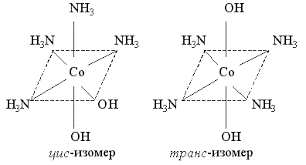
\includegraphics[scale=1.2]{qq6}}
	\end{figure}
\end{itemize}
